%Metroplolis Beamer Theme: https://github.com/matze/mtheme
\documentclass[aspectratio=169, 10pt, dvipsnames, handout]{beamer}
\usetheme{metropolis}
\usepackage{appendixnumberbeamer, lmodern, bookmark,fontawesome}
\usepackage{booktabs}
% \usepackage[sorting=none]{biblatex}
\usepackage[scale=2]{ccicons}
\usepackage{pgfplots}
\usepgfplotslibrary{dateplot}
\usepackage{xspace}
\newcommand{\themename}{\textbf{\textsc{metropolis}}\xspace}
\usepackage{bbm}
\usepackage{tikz, graphicx}
\usepackage{caption}
\usepackage{multicol}
% \usepackage[dvipsnames]{xcolor}
\usepackage{animate}
\usepackage{scalerel,xparse}
\usepackage{amsmath}
\usepackage{subfig}
\usepackage[style=british]{csquotes}

\newcommand*\colourcheck[1]{%
  \expandafter\newcommand\csname #1check\endcsname{\textcolor{#1}{\ding{52}}}%
}
\colourcheck{blue}

\title{Progress update}
% \subtitle{Lab Update}
\date{\today}
\author{Philip Hartout}

% \titlegraphic{\hfill\includegraphics[height=1.5cm]{logo.pdf}}

\hypersetup{
  colorlinks=true,
  linkcolor=orange,
  filecolor=orange,
  urlcolor=orange,
}

\def\signed #1{{\leavevmode\unskip\nobreak\hfil\penalty50\hskip1em
  \hbox{}\nobreak\hfill #1%
  \parfillskip=0pt \finalhyphendemerits=0 \endgraf}}

\newsavebox\mybox
\newenvironment{aquote}[1]
  {\savebox\mybox{#1}\begin{quote}\openautoquote\hspace*{-.7ex}}
  {\unskip\closeautoquote\vspace*{1mm}\signed{\usebox\mybox}\end{quote}}

\titlegraphic{%
  
\includegraphics[width=.2\textwidth]{figures/mlcb-transparent.png}\hfill
  
\includegraphics[width=.2\textwidth]{figures/dbsse-transparent.png}\hfill
  
\includegraphics[width=.2\textwidth]{figures/eth-transparent.png}
}

\makeatletter
\setbeamertemplate{title page}{
  \begin{minipage}[b][\paperheight]{\textwidth}
    \vfill%
    \ifx\inserttitle\@empty\else\usebeamertemplate*{title}\fi
    \ifx\insertsubtitle\@empty\else\usebeamertemplate*{subtitle}\fi
    \usebeamertemplate*{title separator}
    \ifx\beamer@shortauthor\@empty\else\usebeamertemplate*{author}\fi
    \ifx\insertdate\@empty\else\usebeamertemplate*{date}\fi
    \ifx\insertinstitute\@empty\else\usebeamertemplate*{institute}\fi
    \vfill
    \ifx\inserttitlegraphic\@empty\else\inserttitlegraphic\fi
    \vspace*{1cm}
  \end{minipage}
}
\makeatother

\usetikzlibrary{shapes.geometric, arrows}

\tikzstyle{orangebox} = [rectangle, rounded corners, minimum width=2cm, minimum height=0.5cm, draw=black, fill=orange!40]
\tikzstyle{bluebox} = [rectangle, rounded corners, minimum width=2cm, minimum height=0.5cm, draw=black, fill=blue!40]

\tikzstyle{arrow} = [thick,->,>=stealth]


\begin{document}

\maketitle

\begin{frame}[fragile]{Introduction}
  \begin{itemize}
  \item TDA stuff
  \item Perturbations
  \item Next steps?
  \end{itemize}
\end{frame}

\begin{frame}[fragile]{Kernels on persistence diagrams}
  Implemented properly from GUDHI \cite{gudhi:PersistenceRepresentations}.\\
  A number of kernels are available:
  \begin{itemize}
  \item The sliced Wasserstein kernel (approximates Wasserstein similarity between
    PDs and is p.s.d.). \cite{carriere2017sliced}
  \item The persistence weighted Gaussian kernel (slower to compute + approximates).
    \cite{kusano2016persistence}
  \item The persistence scale space kernel \cite{reininghaus2015stable}
    (approximates, is slower as well). \cite{reininghaus2015stable} proves that the
    $p$-Wasserstein distance is not n.s.d.
  \item The persistence Fisher kernel \cite{le2018persistence}. Looks the
fastest and does not approximate any other distance to be p.s.d.
  \end{itemize}
\end{frame}

\begin{frame}[fragile]{Perturbations}
  Nice visualizations
  \begin{figure}%
    \centering
    \subfloat[\centering No noise]{{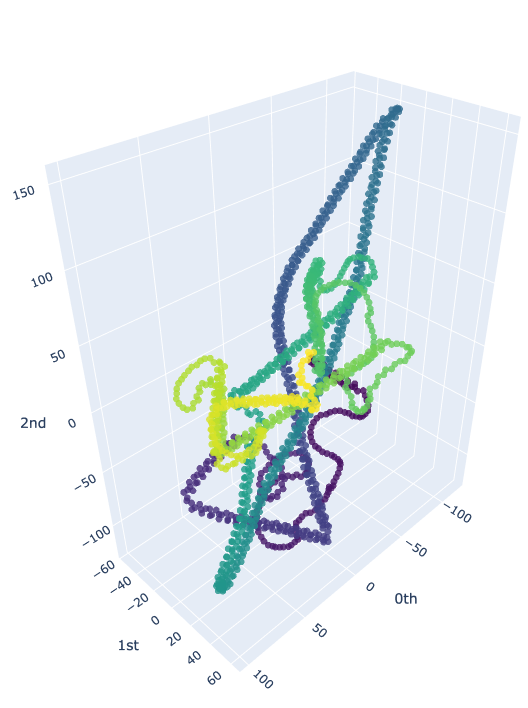
\includegraphics[width=0.2\textwidth]{./figures/base.png}}}%
    \qquad
    \subfloat[\centering 2]{{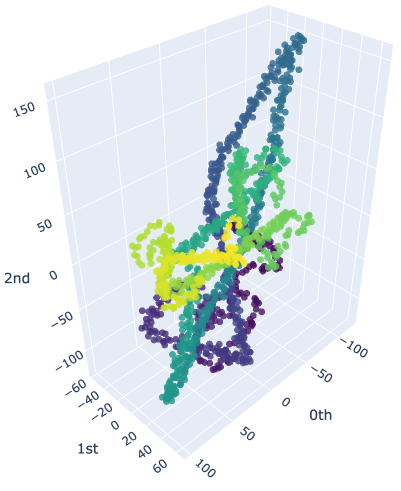
\includegraphics[width=0.2\textwidth]{./figures/std_2.png}
      }}%
    \qquad
    \subfloat[\centering 6]{{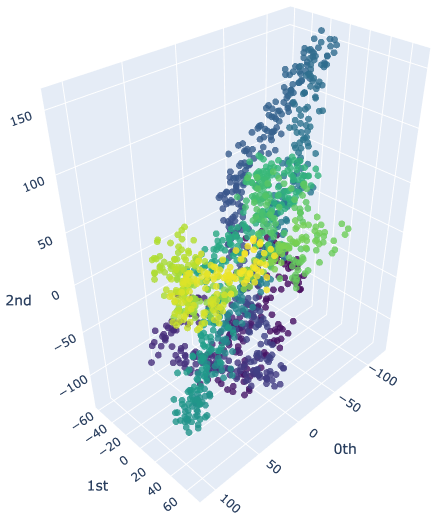
\includegraphics[width=0.2\textwidth]{./figures/std_6.png}
      }}%
    \subfloat[\centering 99]{{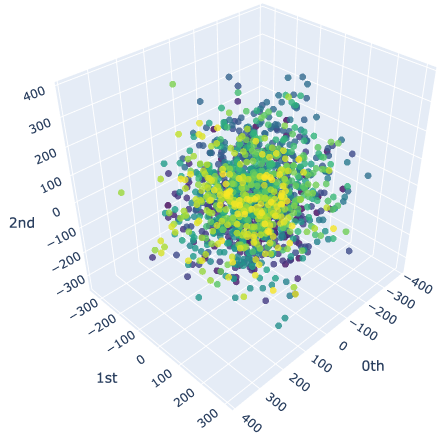
\includegraphics[width=0.2\textwidth]{./figures/std_99.png} }}%
    \caption{Progressive injection of Gaussian Noise}%
  \end{figure}
\end{frame}


\begin{frame}[fragile]{Single experiment}
  \begin{figure}%
    \centering
    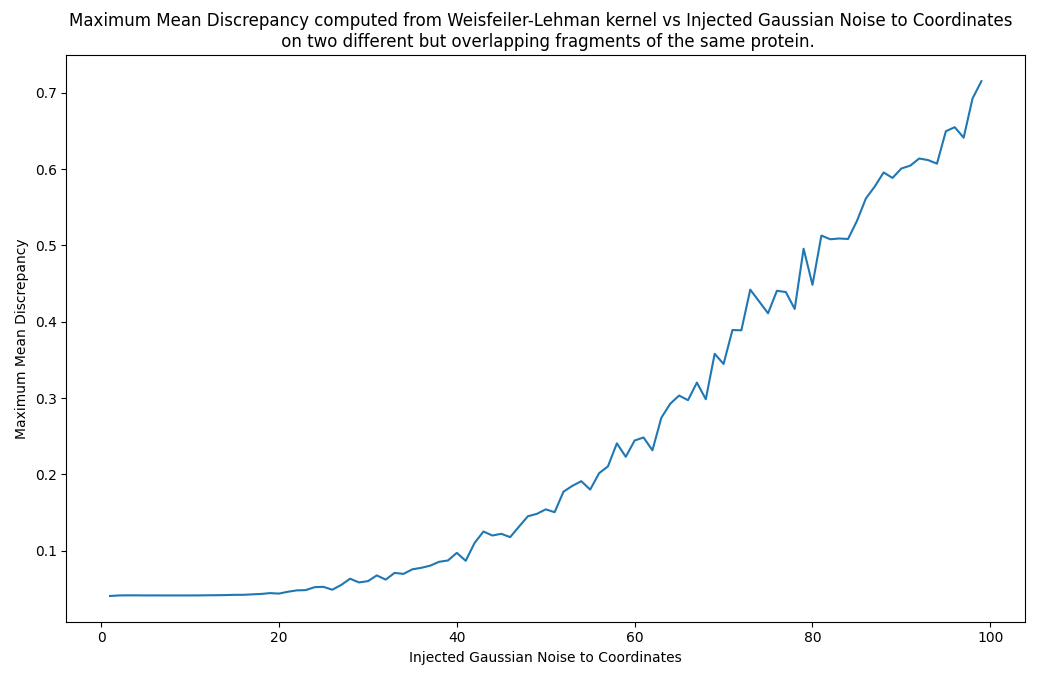
\includegraphics[width=.7\textwidth]{./figures/plot_experiment.png}
    \caption{What happens to the MMD for $\varepsilon=20$?}%
  \end{figure}
\end{frame}

\begin{frame}[fragile]{Multiple experiments varying $\varepsilon$ for the
    $\varepsilon$-graphs}
  \begin{figure}%
    \centering
    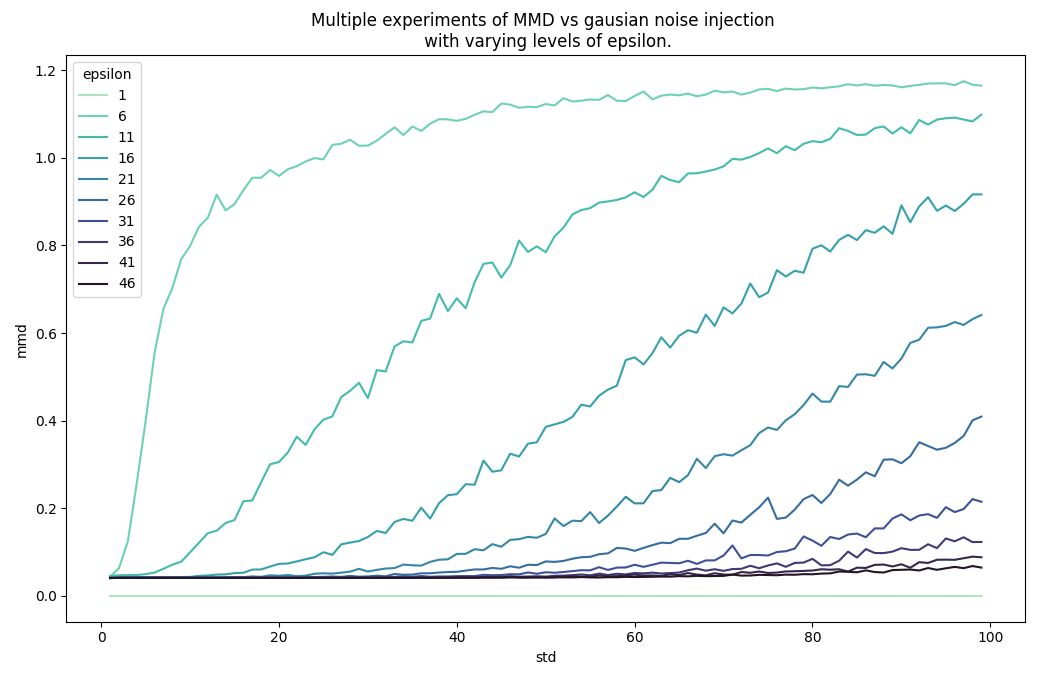
\includegraphics[width=.7\textwidth]{./figures/plot_multiple_experiments.png}
    \caption{What happens to the MMD if $\varepsilon$ varies?}%
  \end{figure}
\end{frame}

\begin{frame}[fragile]{Compressed representations}
  \begin{figure}%
    \centering
    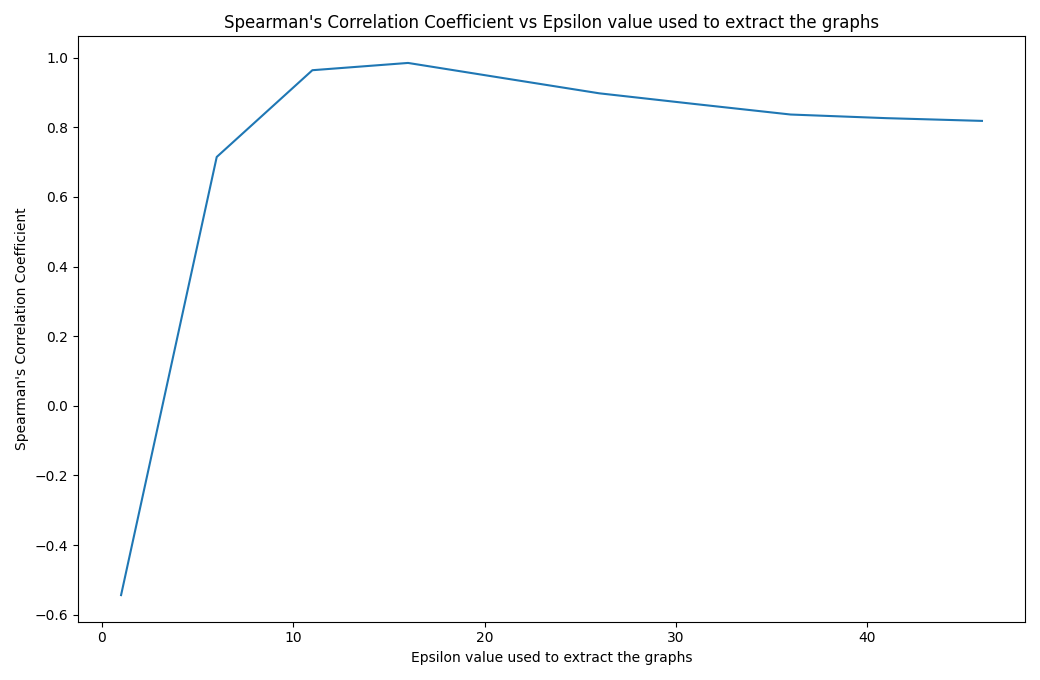
\includegraphics[width=.7\textwidth]{./figures/plot_correlations.png}
    \caption{How can we represent the previous plot in a more compressed way?}%
  \end{figure}
\end{frame}

\begin{frame}[fragile]{Next steps}
  \begin{itemize}
  \item Data version control and better pipelining using dvc
  \item Apply perturbations to subdomain (apply rotation to part of protein)
  \item Clashing descriptors, Ramachandran angles
  \item Non-MMD based meaure. \cite{thompson2022evaluation}
  \item TDA experiments using aforementioned kernel
  \item Actually make progress on background?
  \end{itemize}
\end{frame}


\begin{frame}[allowframebreaks]{References}

  \bibliography{../../thesis/refs.bib}
  \bibliographystyle{abbrv}

\end{frame}

\end{document}
